\chapter{Didaktik und Konferenzen}

In diesem Kapitel wird zunächst Didaktik definiert. Zu der Didaktik werden verschiedene Modelle erläutert. Anschließend werden Didaktische Methoden vorgestellt. Im zweiten Teil dieses Kapitels werden verschiedene Messen und Konferenzen, die sich mit Didaktik beschäftigen vorgestellt. Bei diesen werden die Inhalte, die Ziele und der Umgang mit der Corona-Pandemie der Organisationen vorgestellt.

\section{Didaktik}
 

\subsection{Definition von Didaktik} 

Die Dikdaktik ist die Wissenschaft von der Lehre und der Kunst des Unterrichtens. Das Ziel der Didaktik ist es Lerninhalte abgestimmt auf eine Gruppe auszuwählen. Zu der Auswahl der Inhalte gehört desweiteren die Anordnung der Inhalte sowie das Darstellen der Inhalte.\autocite{Lehner.2019} 
Dabei teilt sich die Didaktik in verschiedene Fachdidaktiken. Diese beschäftigen sich mit einer bestimmten Fachrichtung und wenden die zuvor genannte Didaktik auf diesen Fachbereich an. Dabei teilen sie den Inhalt ihrer Fachrichtung für unterschiedliche Gruppen verständilich ein.\autocite{Lehner.2019} 

\subsection{Das didaktische Dreieck}

\begin{figure}[h]
    \centering
    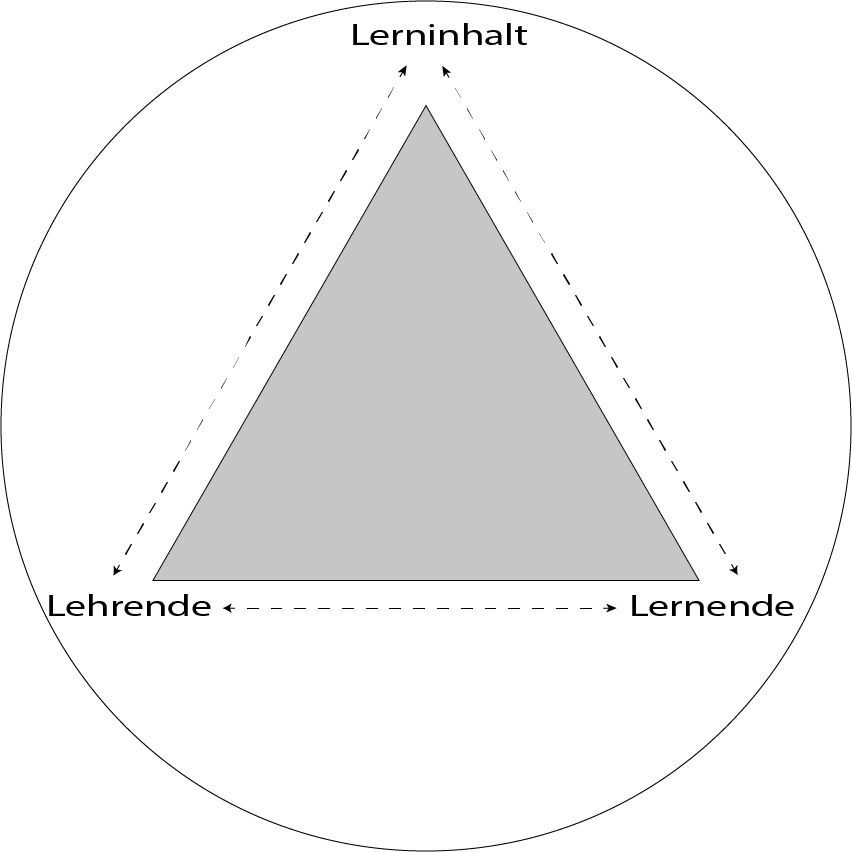
\includegraphics[width=0.7\textwidth]{img/Didaktisches_Dreieck.png}
    \caption[Logo: Learntec]{Logo der Learntec}
    \label{fig: Didaktisches Dreieck}
\end{figure}

Das didaktische Dreieck besteht aus drei Kernelementen. Diese sind der Lernende, der Lehrende und der Lerninhalt. Diese Elemente stehen jeweils in einem Wechselverhältnis und beeinflussen sich daher gegenseitig. 

In Lehner befinden sich die Elemente zusätzlich in einem Kreis. Der Kreis stellt das Umfeld der Elemente dar. 

Der Lernende versucht mit seiner Motivation, seinen Interessen und Voraussetzungen, verschiedene Lerninhalte verstehen. In Martin Lehner werden ebenfalls die soziokulturenne und lerngruppenspezifischen Aspekte durch das Umfeld verdeutlicht.
 Dabei wird er von dem Lehrenden unterstützt. Die Aufgabe des Lehrenden ist es nun die Inhalte dem lernenden verständlich näher zu bringen. Dazu setzt er verschiedene Methoden ein. 

Zudem schränkt der Lehrende die Lerninhalte für den Lernenden ein. Der Lehrende spielt demnach eine Unterstützende aber zentrale Rolle in der Didaktik und bringt die beiden anderen Elemente näher aneinander.

Wichtig ist es, dass sowohl Lerninhalt als auch die angewendeten Methoden auf den Lernenden und seine Eigenschaften und Fähigkeiten abgestimmt werden. 

Der Lerninhalt ist an eine Sache oder an eine Fachrichtung gebunden und ist in sich unabhängig von dem Lehrenden und dem Lernenden.\autocite{Lehner.2019}

\subsection{Das Berliner Modell}
\begin{figure}[h]
    \centering
    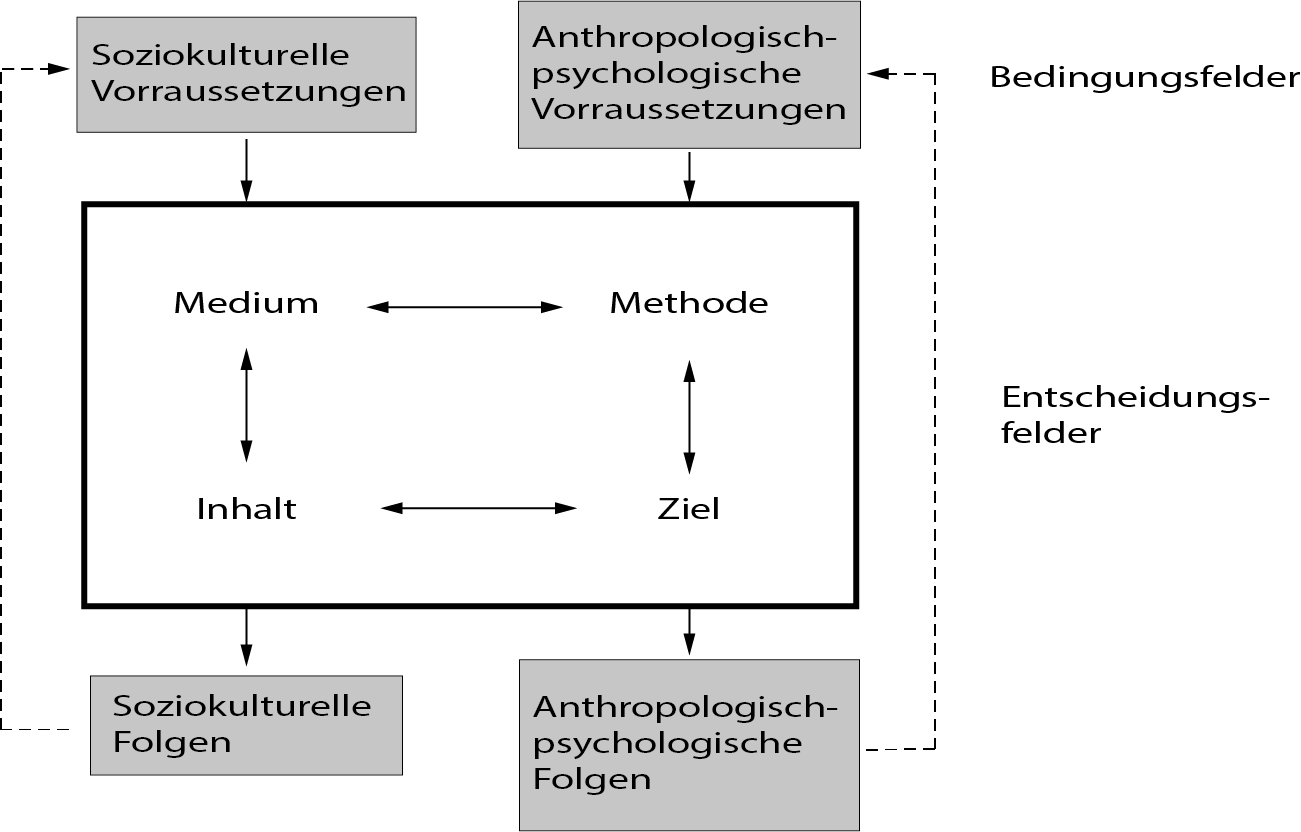
\includegraphics[width=1\textwidth]{img/berlinerModell.png}
    \caption[Grafik: \ac{Berliner Modell}]{Berliner Modell Heimann S56}
    \label{fig:Berliner_Modell}
\end{figure}  
Das Berliner Modell erklärt, \enquote{welche Faktoren im Unterricht eine Rolle spielen und nach welchen Gesichtspunkten diese arrangiert werden sollen, damit nachhaltiges Lernen stattfinden kann}S 55

Die oberen Felder des Modelles stellen die Bedingungsfelder dar. Unter den Anthropogenen und individuellen Vorraussetzungne sind personenbezogenen Eigenschaften der Lernenden zu verstehen. Dazu zählen die Sprache, Vorkenntnisse, sowie die Fähigkeit und der Wille zu lernen. 

Die soziokulturennen Vorraussetzungen sind die Einflüsse auf das Lernen und Lehren. Hiermit sind beispielsweise die Gruppengröße der Lernenden pro lehrenden, die Ausstattung der Organisation und die gesellschaftlichen Interessenlagen. 

Diese Bedinungsfelder können nicht von den Lehrenden beeinflusst werden und bedingen die Entscheidungsfelder, welche sich in der Mitte der Grafik befinden. Die Entscheidungsfelder befinden sich im Einflussbereich des Lehrenden.

Ziele werden gestaltet, um die einen Erreichungsgrad zu erstellen. Anhand dessen kann im späteren Lernverlauf der Erfolg gemessen werden. Diese können zwischen dem Lernenden und dem Lehrenden kommuniziert werden und unterschiedliche Detailgrade aufweisen. 

Inhalt diese entsprechen den Lerninhalten aus dem didaktischen Dreieck. Die Inhalte müssen von dem Lehrenden sinnvoll eingegrenzt werden, um sie den Lernenden näher zu bringen. 

Methode sind die Verbindung zwischen den Lehrenden und dem Lernenden mit denen der Lerninhalt näher gebracht wird. Es gibt viele verschiedene Methoden die von den Lehrenden angewendet werden können. Ein guter Lehrender besitzt eine große Auswahl an Methoden, die ihm das Lehren vereinfachen.

Mit der Hilfe von Medien, wie Beispielsweise einer Tafel, einem Tageslichtprojektor oder Modellen kommuniziert der Lehrende mit dem Lernenden. In der Zeit von Corona werden Folien in online Präsentationen oder Videos eingesetzt, um die Lerninhalte zu visualisieren und damit leichter verständlich zu machen. 

\enquote{Das Berliner Modell der Didaktik bietet Strukturhilfen zur Planung und Analyse von Unterricht}S 57. Dieses Modell wurde später durch das Hamburger Modell voin Schulz erweitert und wird in dieser Arbeit nicht näher betrachtet.

\subsection{Didaktische Methoden}
 Martin Lehner zählt viele Verschiedene Methoden auf. Diese teilen sich in die klassischen Methoden und neue Methoden auf.

 \textbf{Klassische Methoden}
 \begin{itemize}
     \item Lehrvortrag
     \item Lehrgespräch
     \item Diskussion
     \item Einzel-, Partner-, Gruppenarbeiten
 \end{itemize}
 \textbf{Beispiele neuer Methoden}
\begin{itemize}
    \item Flipped Classroom
    \item Projektmethode
    \item Handlungsorientierter Unterricht
    \item Moderationsmethode
\end{itemize}

Der Lehrvortrag erfodert von dem Lehrenden viel ab ist ein Vortrag von diesem der Lernende nimmt dabei eine sehr passive Rolle ein. Eine Steigerung dieser Form ist das Lehrgespräch, welche dem klassischen Schulunterricht entspricht. In dieser Methode werden dem Lernenden von dem Lehrenden Fragen gestellt. Diese Fragen führen den Unterricht weiter, fragen wissen ab oder klären offene Fragen. 

Die Diskussion ist eine etwas kaotischere Form des Lehrgespräches. Der Lehrende nimmt eine lenkende Rolle ein. Die Diskussion wird von den Lernenden gefüllt. 

In Einzel-, Partner und Gruppenarbeiten werden den Lernenden kleinere Aufgaben gegeben, welche sie in Eigenarbeit bearbeiten. 

In der neuen Methode des Flipped Classroom werden den Lernenden Aufgaben gegeben, welche sie selbständig bearbeiten. Zur Unterstützung dienen Videos. Die Aufgabe des Lehrenden ist es bei Schwierigkeiten, offenen Fragen und Unversändlichkeiten zu untersützen. 

In der Projektmethode arbeiten die Lernenden in einem begrenzten Zeitraum an einem Thema. In dieser Zeit setzten sie sich oft mit verschiedenen überschneidenden Fächern auseinander und verstehen die Zusammenhänge dieser. 

\subsection{Zusammenfassung}


\section{\ac{MOBTS}}


\begin{figure}[h]
    \centering
    
\includegraphics[width=0.8\textwidth]{img/mobtslogo.png}
    \caption[Logo: \ac{MOBTS}]{Logo der \ac{MOBTS}}
    \label{fig:LOGO_MOBTS}
\end{figure}

Die \ac{MOBTS} hat sich als Mission gesetzt die Qualität des Lehrens und des Lernens über alle Managementdisziplinen zu verbessern.\autocite{MOBTS.452021} 

Die Vision der \ac{MOBTS} ist es Pädagogen aus verschiedenen Stufen ihrer Laufbahn zusammenzubringen. Das Ziel ist es, dass diese voneinander lernen und gegenseitig lehren können.\autocite{MOBTS.452021} 

Zu den Werten der \ac{MOBTS} zählen gegenseitiger Respekt, die persönliche Weiterentwicklung des einzelnen, das Teilen von Ideen und verschiedene Lehrfähigkeiten mit anderen.\autocite{MOBTSExecutiveCommitee.432021} 

Die Society unterstützt und leitet seine Mitglieder beim lehren und lernen indem sie es Ermöglicht Lehr- und Lernressourcen, Best Practices, Innovation teilt. Dies wird durch Konferenzen und Publikationen umgesetzt.\autocite{MOBTS.452021}// hier die richtige quelle einffügen Die sowohl im nationalen als auch internationalen Umfeld stattfinden. 

Die \ac{MOBTS} als Society hat einen klaren Aufbau mit einem Vorstand aus elf Personen bestehenden. Dieser wird in dem jährlichen 'annual business meeting' gewählt. Die Mitglieder der Society haben die Möglichkeit Papers zu veröffentlichen, an der jährlichen Konferenz und an internationalen Konferenzen teilzunehmen.\autocite{MOBTS.452021} 

An den Konferenzen können nur Mitglieder der Society teilnehmen. Die Mitgliedschaft muss jährlich verlängert werden und kostet für Studenten 35 Dollar und ansonsten 55 Dollar.\autocite{MOBTS.432021e} Mit diesem Geld werden die Konferenzen finanziert. Die Society ist eine non-profit Organisation.  

Die erste Konferenz der \ac{MOBTS} fand 1974 in der Stanford University statt. Im Jahr 1995 fand dann die erste internationale Konferenz in Australien statt.\autocite{MOBTS.432021c} Heute besteht die Society aus über 500 Mitgliedern und hat bereits zahlreiche Konferenzen veranstaltet.\autocite[Vgl. Minute 13]{MOBTS.432021b}

Die letzte Konferenz fand 2020 Aufgrund der Corona Pandemie erstmals in einem digitalen Umfeld statt. Hierzu wurde die Anwendung Zoom verwendet. Die Teilnehmer konnten an verschiedenen Sessions, von denen einige gleichzeitig stattfanden, teilnehmen. Hierzu musste sich im Vorhinein angemeldet werden.\autocite{MOBTS.432021d}  Dabei gab es die Möglichkeiten sich an Diskussionen zu beteiligen als und Vorträgen zu zuhören. Diese Version der Konferenz ist ebenfalls für das Jahr 2021 geplant. 

Weitere Anpassungen an die Corona Pandemie ist ein YouTube Kanal, auf welchem für alle frei zugänglich Vorträge verschiedener Mitglieder und Einblicke in die \ac{MOBTS} geteilt werden.\autocite{MOBTS.432021} 

2021 wird die \ac{MOBTS} an der DHBW stattfinden. In dieser Arbeit wir weiter auf die \ac{MOBTS} und die Planung der Konferenz an der DHBW eingegangen.

\section{\ac{AOM}}
\begin{figure}[h]
    \centering
    
\includegraphics[width=1.3\textwidth]{img/th.jpg}
    \caption[Logo: AOM]{Logo der \ac{AOM}}
    \label{fig:LOGO AOM}
\end{figure}
Die Mission der \ac{AOM} ist es eine lebendige und sich unterstützende Gemeinschaft aus Wissenschaftlern aufzubauen. Diese Gemeinschaft soll es den Mitgliedern ermöglichen sich zu vernetzen und gemeinsam an Ideen zu forschen.\autocite{AOM_CMS.432021b} 

Die Vision der \ac{AOM} hat das Ziel die Welt zu inspirieren und durch Forschung  und Lehre über Management und Organisationen zu verbessern. \autocite{AOM_CMS.432021b}

Die \ac{AOM} ist eine Community die sich mit dem Lernen und dem Lehren beschäftigt. In dieser Community sind sowohl Studenten, Professoren als auch Praktikanten vertreten.\autocite{AOM_CMS.432021d}

In der jährlichen Konferenz der \ac{AOM} geht es um aktuelle Themen zu den Entwicklungen in der Forschung. Während der Konferenz finden verschiedene Präsentationen statt und Researchs werden  präsentiert.\autocite{AOM_CMS.432021b} 

Die \ac{AOM} wurde bereits im Jahr 1936 gegründet und hat heute mehr als 20 000 Mitgliedern in über 120 verschiedenen Ländern.\autocite{AOM_CMS.432021b} 

Die \ac{AOM} 2020 fand in einem digitalen Format statt. Die Sessions teilen sich in live und im voraus Aufgenommene Sessions auf. Während die aufgenommenen Sessions bereits im Vorhinein angeschaut werden können und dazu Fragen eingereicht werden können finden die live Sessions in Zoomeetings mit bis zu 500 aktive Teilnehmern statt. \autocite{AOM_CMS.432021} 

Im Zoom Umfeld gibt es einen Präsentator, welcher einen Vortrag hält. Zu diesem Vortrag können anschließend Fragen gestellt werden. Des Weiteren wird die Breakout-Funktion von Zoom genutzt, um in kleineren Gruppen zu diskutieren. Alle Sessions können aufgenommen werden und somit im Nachhinein erneut angeschaut werden. \autocite{AOM_CMS.432021c} 

Auch im Jahr 2021 ist eine digitale Konferenz geplant. \autocite{AOM_CMS.432021d}  Ein Teil des Jährlichen Konferenz ist die Techaching and Learning Conferenc also die Lehren und lernen Konferenz. In diesem Teil der Konferenz wird besonders auf das Lehren und das lernen von Inhalten eingegangen.


\section{Die LEARNTEC}
\begin{figure}[h]
    \centering
    
\includegraphics[width=0.6\textwidth]{img/logolearn.png}
    \caption[Logo: Learntec]{Logo der Learntec}
    \label{fig: LOGO LEARNTEC}
\end{figure}
Die Learntec ist eine Bildungsmesse die sich mit dem digitalen lernen beschäftigt. Dabei werden die Bereiche Schule, Hochschule und Beruf abgedeckt. Zu diesen Bereichen gibt es für die Gruppe angepasste Informationen und Ansätze zur digitalen Bildung. \autocite{KarlsruherMesseundKongressGmbH.3232021} 

Die erste Learntec Messe fand 2016 statt und ist somit die jüngste vorgestellte Organisation. Das Interesse an dieser Messe steigt seitdem stark an.
\autocite[Vgl.]{KarlsruherMesseundKongressGmbH.3232021} 

In dem Jahr 2020 fand die Messe in Karlsruhe statt und hatte über 400 verschiedene Aussteller sowie über 15 000 Besucher. Auf der Messe wurden über drei Tage verteilt verschiedene digital unterstützte Lernmethoden vorgestellt. Zu diesen zählen die Gamification, Virtual Reality, mobiles lernen und lernNuggets.  (diese Themen vorstellen?) \autocite{KarlsruherMesseundKongressGmbH.3232021}

Gamification ist Beispielsweise das Aufbereiten von Lerninhalten, sodass diese als spielerische Elemente in einen Zusammengebracht werden. Dieses Vorgehen soll die Motivation steigen und Verhaltensänderungen hervorbringen. \autocite{Prof.Dr.OliverBendel.7.1.2019}

Die Pandemie hat dazu geführt, dass online Vorträge von Experten und Diskussionsrunden über das Digitale lernen stattfinden. Die Themen in diesen Vorträgen passen sich den aktuellen Umständen an und handeln von der Hybriden lehre, also das Unterrichten Vorort an Schulen und online Unterricht. Des weiteren wird das Digitalpaket Schule vorgenommen. \autocite{KarlsruherMesseundKongressGmbH.3232021b} 

Weitere Themen der Messe sind die Hardware und Ausstattung sowie Wissensmanagement und Bildungsmanagement. Des weiteren verfügt die Lerntec über einen Podcast in dem über Themen im Bereich digitalen Lernen gesprochen wird.\autocite{KarlsruherMesseundKongressGmbH.432021} 

Auf der Webseite der Learntec gibt es weitere Inhalte zu den genannten Themen. 
